\documentclass{beamer}
\usetheme{Madrid}
\usecolortheme{default}

\usepackage[utf8]{inputenc}
\usepackage{booktabs}
\usepackage{array}
\usepackage{colortbl}
\usepackage{graphicx}
\usepackage{tikz}
\usetikzlibrary{positioning}
\definecolor{primaryblue}{RGB}{0,100,200}  % Blue shade for primary elements
\definecolor{successgreen}{RGB}{0,150,80}  % Green shade for success/highlights
\definecolor{errorred}{RGB}{200,50,50}     % Red shade for poor performance

\title{Geometrical Reconstruction using Acoustic Tactile Sensing}
\author{Georg Wolnik}
\institute{TU Berlin - Robotics and Biology Department}
\date{\today}

\begin{document}

% Title slide
\begin{frame}
\titlepage
\end{frame}

% ──────────────────────────────────────────────────────────────
% NEW SLIDE: Research Question + Processing Pipeline Visualization
% ──────────────────────────────────────────────────────────────
\begin{frame}{End-to-end Project Pipeline}

\begin{center}
\textbf{Core Process + Iterative Improvement}
\end{center}

\vspace{0.5cm}

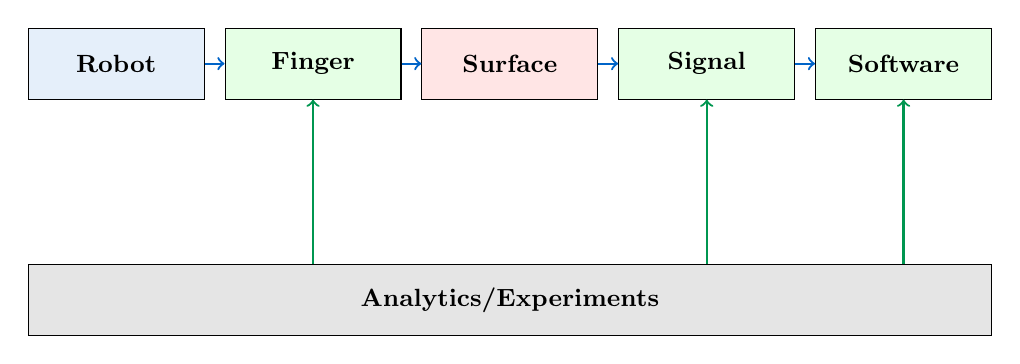
\begin{tikzpicture}[scale=1.0, node distance=1.6cm, every node/.style={font=\small}]
    
    % === Upper line – 5 boxes ===
    \node[draw,fill=primaryblue!10,minimum height=0.9cm,text width=2cm,align=center] (u1) at (0.5,4) {\textbf{Robot}};
    \node[draw,fill=green!10,minimum height=0.9cm,text width=2cm,align=center] (u2) at (3,4) {\textbf{Finger}};
    \node[draw,fill=red!10,minimum height=0.9cm,text width=2cm,align=center] (u3) at (5.5,4) {\textbf{Surface}};
    \node[draw,fill=green!10,minimum height=0.9cm,text width=2cm,align=center] (u4) at (8,4) {\textbf{Signal}};
    \node[draw,fill=green!10,minimum height=0.9cm,text width=2cm,align=center] (u5) at (10.5,4) {\textbf{Software}};
    
    \draw[->,thick,primaryblue] (u1) -> (u2);
    \draw[->,thick,primaryblue] (u2) -> (u3);
    \draw[->,thick,primaryblue] (u3) -> (u4);
    \draw[->,thick,primaryblue] (u4) -> (u5);
    
    
    % === Lower line – One wide box ===
    \node[draw,fill=gray!20,minimum height=0.9cm,text width=12cm,align=center] (l1) at (5.5,1) {\textbf{Analytics/Experiments}};
    
    
    % === Arrows from lower to upper ===
    \draw[->,thick,successgreen] (u2 |- l1.north) -> (u2.south);
    \draw[->,thick,successgreen] (u4 |- l1.north) -> (u4.south);
    \draw[->,thick,successgreen] (u5 |- l1.north) -> (u5.south);
\end{tikzpicture}
\end{frame}
% ──────────────────────────────────────────────────────────────
% FINAL CONCLUSION – SHORT, STRONG, MEMORABLE (one slide only)
% ──────────────────────────────────────────────────────────────
\begin{frame}{Conclusion \& Look Ahead}

\begin{enumerate}[1.]
    \item Validate acoustic finger setup
    \item Apply greater force with finger on surface
    \item Adjust angle of finger to increase surface contact area
    \item Start with static recordings moving slowly to dynamic ones
    \item Balance out dataset distribution
\end{enumerate}

\end{frame}

\end{document}